\documentclass[twoside]{article}
\usepackage{ecj,palatino,epsfig,latexsym,natbib}
\usepackage{graphicx}
\usepackage[ruled,vlined]{algorithm2e}
\usepackage{amsmath,amssymb} 
\usepackage{tikz}
\usepackage{color}		% this package has a variety of color options
\usepackage[showchanges]{seanmacros}

%\smartqed  % flush right qed marks, e.g. at end of proof

\newtheorem{theorem}{Theorem}
\newtheorem{definition}{Definition}

\newcommand{\IR}{\mathbb{R}}

%% Some Usefull colors
\xdefinecolor{oiB}{rgb}{0.22,0.52,0.72}
\definecolor{oiG}{rgb}{.298,.447,.114}
\xdefinecolor{hlblue}{rgb}{0.0,0.0,0.7}
\xdefinecolor{gray}{rgb}{0.5, 0.5, 0.5}
\definecolor{lightgrey}{gray}{0.95}
\xdefinecolor{darkGray}{rgb}{0.3, 0.3, 0.3}
\xdefinecolor{darkerGray}{rgb}{0.2, 0.2, 0.2}
\xdefinecolor{rubineRed}{rgb}{0.89,0,0.30}
\xdefinecolor{irishGreen}{rgb}{0,0.60,0}	

%% Colorblind friendly colors
\xdefinecolor{darkCB1}{rgb}{0.2873239, 0.7098592, 0.3971831}
\xdefinecolor{darkCB2}{rgb}{0.5464789, 0.3971831, 0.4507042}
\xdefinecolor{darkCB3}{rgb}{0.4647887, 0.2760563, 0.5718310}
\xdefinecolor{lightCB1}{rgb}{0.4047619, 1.0000000, 0.5595238}
\xdefinecolor{lightCB2}{rgb}{0.7698413, 0.5595238, 0.6349206}
\xdefinecolor{lightCB3}{rgb}{0.6547619, 0.3888889, 0.8055556}

%% Common colors, but not colorblind friendly
\definecolor{darkblue}{rgb}{0.0, 0.0, 0.7}
\definecolor{darkred}{rgb}{0.8, 0.0, 0.0}
\definecolor{darkgreen}{rgb}{0.0, 0.6, 0.0}


%% do not add any other page- or text-size instruction here

\parskip=0.00in

\begin{document}

\ecjHeader{x}{x}{xxx-xxx}{201X}{Analysis of Simple Novelty Search}{R.P. Wiegand}
\title{\bf Preliminary Analysis of Simple Novelty Search}  

\author{\name{\bf R. Paul Wiegand} \hfill \addr{wiegandrp@winthrop.edu}\\ 
        \addr{Department of Computer Science \& Quantitative Methods\\
        Winthrop University, Rock Hill, SC, 29733, United States}
}

\maketitle

\begin{abstract}
%TBD 200 words
Novelty search is a powerful tool for finding diverse sets of objects in complicated spaces.  Recent experiments on simplified versions of novelty search introduce the idea that novelty search happens at the level of the archive space, rather than individual points.  The sparseness measure and archive update criterion create a process that is driven by a two measures:  spread out to \emph{cover} the space, while trying to remain as efficiently \emph{packed} as possible, metrics inspired by $k$ Nearest Neighbor theory.  

In this paper, we generalize previous simplifications of novelty search to include traditional population  $(\mu, \lambda)$ dynamics for generating new search points, where the population and the archive are updated separately.  We provide some theoretical guidance regarding balancing mutation and sparseness criteria and introduce the concept of \emph{saturation} as a way of talking about fully covered spaces.  We show empirically that claims that novelty search is \emph{inherently} objectiveless are incorrect.  We leverage the understanding of novelty search an optimizer of archive \chl{$\;\;\;\;$R1C2}{}{coverage} suggest several ways to improve the search, and we demonstrate one simple improvement\,---\,generate some new points directly from the archive rather than the parent population.
\end{abstract}

\begin{keywords}
novelty search, 
quality diversity,
convergence,
k nearest neighbors.
\end{keywords}

%====================================================================================
\section{Introduction}
\label{sec:introduction}

Though evolutionary computation can be an effective problem solver \citep{ec:DeJong2006,ec:Mitchell97,ec:Michalawicz96,ec:Goldberg89,ec:Holland75}, these biologically-inspired approaches are also applied to tasks other than traditional optimization.  Evolutionary algorithms (EAs) are now used for a variety of creative endeavors from evolving computer programs \citep{ec:LangdonPoli2002,ec:Banzhaf1998,ec:Koza1992} 
 to discovering faults \citep{HanesWiegand2019tor,Mourad2000srds} to producing art \citep{cs:Dreher2014,Secretan2008chi,ec:Romero2007,bio:Dawkins1996}.  In fact, there is an entire subdiscipline of evolutionary computation dedicated to its ability to generate, create, and innovate \citep{ec:Goldberg2002}.  Unfortunately, there is little foundational analysis for such applications.

\emph{Quality diversity algorithms} \chl{$\;\;\;\;$R2C6, R3C12, R3C2, R3C8}{}{\citep{Fontaine2021corr,Choi2021gecco, FontainEtAl2020icog,Nordmoen2020corr,CullyDemiris2017corr,MouretClune2015preprint} use the innovating mechanisms in evolutionary methods to try to saturate the search space by spreading out to find a variety of solutions.} One of the most aggressively advocated methods is so-called, \emph{Novelty Search} \citep{StanleyLehman2015,Lehman2013gecco,LehmanStanley2011cec,LehmanStanley2008ssls}\chl{$\;\;\;\;$R3C8}{}{, which attempts to produce \emph{different kinds} of results (in general), rather than results that optimize an external objective function.}  The motivation behind novelty search is that for certain complex spaces, it may be better to \emph{ignore} the optimization objective and instead \emph{explore} the space by finding objects that are increasingly ``different'' from those that the search process has encountered before.  Though perhaps counter intuitive, novelty search has been surprisingly effective at finding good solutions to a number of challenging problems without even looking for those solutions explicitly.  Examples of novelty search successes include discovering effective grasping behaviors for highly articulated robotic arms \citep{Huang2014cica}, unsupervised feature learning for deep networks \citep{Szerlip2015cai}, discovery of sophisticated gaits for quadruped locomotion \citep{Morse2013acgec}, and goal-seeking in complex multiagent simulations \citep{Lehman2011ecj}.

Advocates of these methods have proposed three critical ideas for \emph{why} novelty search can succeed in such spaces.  The first premise is that novelty search avoids being deceived by local optima since it ignores an external objective in favor of a novelty metric \citep{Lehman2011ecj}.  This is predicated on the claim that novelty search ``\emph{diverges}'' rather than converges.  Second, novelty search tends to be applied when using generative representations \citep{LehmanStanley2008ssls} to encourage a process referred to in the literature as ``complexification'' \citep{StanleyMiikkulainen2004jair}.  Complexification is the systematic and steady increase of complex representations via evolutionary search, and this in conjunction with a divergent search will lead to surprising and nuanced discoveries.  Third, using diversity measures within the true solution space (e.g., agent behaviors) rather than the genotype space allows novelty search to discover ''interesting`` areas of that behavior space.  

While sometimes effective, there's little foundational understanding for whether or how these speculations (or others) lead to success nor much in the way of guidance for how to \emph{improve} novelty search.  Very recently \citet{Doncieux2020gecco,Doncieux2019gecco} have presented a reinforcement learning based formal framework for approaching questions about novelty search.  They use their formalism to suggest hypotheses, which they test empirically and conclude that novelty search mechanisms can be effective at spreading out in behavior space, suggesting that they may be capable of ``uniform sampling'' of that space.  The authors of those studies repeat claims that these algorithms are divergent.  \chl{$\;\;\;\;$R2C2}{}{A slightly older empirical study of novelty search methods \cite{Gomes2015gecco} examines several key parameters of novelty search including the types of archives used (none, novelty, and random), size of the neighborhood used for sparseness calculations, several methods for how fitness and novelty metrics are used during selection, and several variations for the underlying evolutionary algorithm used.  This work included complex algorithms on a maze navigation task, and while it \emph{does} provide real-world advice about how mutation can relate to these choices, it doesn't really address the core behaviors of the algorithm nor whether or not fundamental claims about the algorithm are true.} 

\chl{$\;\;\;\;$R2C6}{}{Quality diversity (QD) methods include different approaches than novelty search.  One well-established alternative are so-called \emph{MAP-Elite} methods \citep{Choi2021gecco,Nordmoen2020corr,Flageat2020corr}.  There are two relevant differences between canonical novelty search and MAP-Elite methods.  The first is that unlike traditional novelty search, MAP-Elites \emph{does} use the external objective function to make selection decisions.  Diversity measures are used to make sure the population / archive spreads out in the space.  The second is that in most applications of MAP-Elites, the population itself is the archive unlike typical applications of novelty search.  Part of our analysis in Section~\ref{subsec:psnsea:improve} will address this point.}

\chl{$\;\;\;\;$R3C2}{}{There are many other types of QD methods, as well.  Some rely on the use of second order information about the problem (e.g., derivatives or gradients) \citet{Fontaine2021corr}, while others represent diversity maintenance mechanisms in traditional evolutionary algorithms, such as crowding \citet{Goldberg1987icga}.  \citep{CullyDemiris2017corr} attempt to provide a general framework to place most, or all of QD methods.  Chiefly, there appears to be a substantive difference in philosophy between approaches in which the external fitness objective is used to guide search dynamics (such as MAP-Elites) and those in which the external fitness objective is ignored for the purposes of search behavior (such as traditional novelty search).  Our focus is on the latter group of methods.}

Are \ch{}{the general claims about novelty search true}?  If not, when are they true?  In this paper, we begin at the top by \ch{}{simplifying the algorithm and problem domain then} looking more closely at the claim that novelty search has no objective, and that it is a ``divergent'' search process \citep{Lehman2016frai,Lehman2015gecco,StanleyLehman2015}\chl{R3C1}{}{}.  This paper isolates the claim as to whether novelty search is inherently objectiveless, and we say nothing at all about complexification or discovery in behavioral spaces.  Moreover, our results do not in any way invalidate the success of novelty search, rather we seek to complement existing research by providing more insight into how these searchers work and how to make principled choices regarding some search parameters.  The goal is to be able to build \emph{better} novelty search algorithms.

To that end, we propose an alternative view of novelty search where the space being searched is not the solution space (e.g., behaviors) but is rather a space of \emph{archives} of potential solutions.  We take inspiration from $k$ nearest neighbor theory to provide a formalization of this idea, conduct empirical analyses using measures based on that formalization, and provide a preliminary theoretical framework for understanding how such a search process works.  Our analysis begins with an extremely simple formulation of novelty search that consists only of the so-called \emph{sparseness} criterion and an archive, and we then relax this by adding a population separate from the archive.  Some preliminary empirical results of this work appear in \citet{Wiegand2020flairs} and \citet{Wiegand2021flairs}, though this article expands on these empirical results and also adds some theoretical guidance.  All experiments in this paper are unique to the present work, though a few replicate experiments from those previous works.  We will be clear where there are overlaps.

\chl{R1C2}{}{We borrow and revise well-known metrics from $k$-NN theory \citet{Clarkson1999dcg} to define $\epsilon$-coverage and $\epsilon$-packing over sets (See Section~\ref{subsec:knn} for the formal definition). We find that novelty search drives the archive toward increasingly better $\epsilon$-covers of the solution space while also trying to optimize the $\epsilon$-packing of the archive.}  Simple variants of novelty search that employ the traditional mechanisms can and do converge, whether or not the space is bounded.  Moreover, local convergence to suboptimal archives is possible.  Understanding this allows us to give some constructive suggestions for how to apply novelty search more effectively: it is essential to balance the mutation rate and the minimum sparseness criterion appropriately, there may be value in selecting some parents directly from the archive, and it may be useful to use convex hull estimates of the archive from which to draw future search points.

\chl{R1C1}{}{In part, much of what any quality diversity method does can be seen through the lens of random sampling theory.  Standard evolutionary algorithms use initialization and genetic operators such as mutation to sample \emph{different} parts of the space \citet{ec:DeJong2006}, and Monte Carlo sampling methods are often used to reduce uncertainty.  Indeed, traditional reinforcement learning methods have been successfully combined with stochastic local search mechanisms by leveraging the fact that these local search methods provide different kinds of sampling of the local space (i.e., a kind of novely) \citet{Boyan1998aaai}.  We will provide a short discussion of the relationship between novelty and uncertainty minimization in the conclusion.}


%====================================================================================
\section{Technical Approach}
\label{sec:approach}

%------------------------------------------------------------------------------------
\subsection{Sparseness and Archives}
\label{subsec:sparseness}

The concept of ``novelty'' in traditional novelty search is enforced by a metric designed to measure the \emph{sparseness score} of a point with respect to a group of points.  Specifically, the sparseness of some candidate object $y$, $\rho_y$, is computed as the average distance to the $k$ nearest neighbors in some set $A$:
%
\begin{eqnarray}
  \rho_y := \frac{1}{k} \sum_{i=1}^{k} \delta\left( x^A_i, y\right),
  \label{eqn:sparseness}
\end{eqnarray}

\noindent where $x^A_i$ is the $i^{th}$ closest point in set $A$ to $y$ and $\delta$ is some kind of distance calculation.  In other words, $\rho_y$ is the average distance between some point $y$ and the $k$ nearest neighbors to that point in some set $A$.  Though perhaps a misnomer, we keep this term since it is consistent with the literature.  For traditional novelty search, this sparseness score is used in two ways.  

First the sparseness score is used as a type of fitness value for evolution.  Points that have larger scores\,---\,more distant from nearby points in some set\,---\,are more fit.  For selection, this set is typically the population, and it can be used for parent and/or survival selection.  It is also possible to also explore the idea of using the archive as the baseline set for selection, and we explore this idea in Section~\ref{subsec:psnsea:improve}.

The second way the score is used is as an update mechanism for an archive of points the search is maintaining:  Novelty search adds individuals to the archive only if their sparseness over that archive is above a certain threshold, $\rho_{min}$.  In this way, the archive grows and begins to contain more and more ``novel'' candidate solutions in the sense that they are \emph{different} from one another as defined by the sparseness score.

Though there are many choices for search operators and selection, the rest of the method is essentially an evolutionary algorithm \citep{ec:DeJong2006}.  The idea that the archive continues to expand with novel search points as search proceeds is what motivates the claim that novelty search diverges.  To be clear, this paper takes no position as to whether or not divergence in novelty search is an appropriate goal; we merely explore an existing claim to determine whether or not it is generally true that novelty search inherently diverges rather than converges.  It is very clear that the original researchers who composed novelty search intended the search to diverge \citep{Lehman2016frai,Lehman2015gecco,StanleyLehman2015}.


%------------------------------------------------------------------------------------
\subsection{Archive-Based Searches}
\label{subsec:archive}

In traditional uses of an evolutionary algorithm, individuals in the population represent candidate solutions to a problem.  The search space is the set of candidate solutions to the problem, population members represent potential solutions, and the EA searches that space to find the a good solution.  Given this perspective, it is easy to understand why novelty search \emph{appears} to be objectiveless:  though individuals may be encoding candidate solutions, the algorithms completely ignore the optimization objective associated with that candidate solution with respect to some external problem.  One can imagine search diverging in the sense that increasingly different candidate solutions are progressively proposed in an ever-growing archive, and the direction of that growth is not at all influenced by the problem's objective.  

However, there are alternative ways to understand archive-based searches.  Specifically, some search methods are designed to search a \emph{space of archives}, not individual points.  The multiobjective optimization problem is typically formulated to find an approximation of the Pareto non-dominating \emph{set} for some solution space \citep{SeadaDeb2018moo,Zitzler2012,Zitzler2000ecj}.  Further, \emph{cooptimization} problems, to which coevolutionary algorithms are often applied, are supersets of multiobjective optimization problems.  In cooptimization, the goal is to simultaneously identify the set of underlying objectives and produce a set obeying some solution concept \citep{FiciciPollack2001ecal,BucciPollack2002foga,Popovici2012,Ficici2008mpsn}.  That solution concept may be Pareto-based, but there other concepts (e.g., sets that approximate mixed Nash equilibria).

We take the position that novelty search is, in fact, \emph{not} searching the space of candidate problem solutions being represented by individuals in the population.  Instead, it is searching the space of \emph{novel archives}.  The true goal of this search is to develop an archive that spreads out in some space while also keeping the points in that archive not too close together.  These two notions can be formalized by using slightly modified versions of the concepts of \chl{$\;\;\;\;$R1C2}{}{\emph{coverage}} and \emph{packing} from $k$ nearest neighbor ($k$-NN) theory.  In Section~\pageref{subsec:knn} we will define these terms more formally, and we will also describe some heuristic approximations for measuring these in empirical studies.

In this article, we will consider two variations of novelty search:  \emph{simple novelty search} and \emph{population-based simple novelty search}.  For the latter, we will consider both when population selection uses the population for the baseline sparseness measure, as well as when it uses the archive.   In the former, the population and the archive is the same.  We will also provide some simple formalisms regarding  simple novelty search in bounded Hamming spaces.

%------------------------------------------------------------------------------------
\subsection{The Simple Novelty Search EA}
\label{subsec:sns}

We start with a minimalist understanding of novelty search that has only three major components: a genetic operator, an archive, and an update rule.  While the archive is a set of points, this minimalist algorithm cannot be said to have a population \textit{per se}.  Or, perhaps more precisely, the population \emph{is} the archive (and vice-versa).  The purpose of considering this minimalist approach is to understand the fundamental role of the archive's update mechanism.  Informally, the algorithm works as follows.  A parent is selected uniformly at random from within the archive itself, copied then mutated to produce a child.  The child's sparseness is measured against the archive using Equation~\ref{eqn:sparseness}.  If that value is greater than some selected $\rho_{min}$, then the child is added to the archive.  This is repeated until some termination criterion is met.  The pseudocode for this is replicated below; it first appeared in \citet{Wiegand2020flairs}.

\begin{algorithm}[h]
  \SetAlgoLined
  \DontPrintSemicolon 
  \SetKwInOut{Input}{input}
  \SetKwInOut{Output}{output}
  
  \Input{$\rho_{min}, k,$ termination criterion}
  \Output{$archive$}\;
    
  initialize individual $x$\;
  $archive$ = $\{x\}$\;
  \While {not reached termination condition} {
    draw $parent$ uniformly at random from $archive$\;
    $child$ = mutate(copy of $parent$)\;
    $\rho = \mbox{sparseness}(child, archive, k)$\;
    \If {$\rho \geq \rho_{min}$} {
      $archive = archive \cup \{child\}$\;
     }
  }
  \caption{Simple Novelty Search Evolutionary Algorithm (SNSEA)}
\end{algorithm}

For this article, we consider $k=3$ for the sparseness computation.  The termination criterion is simply a maximum number of generations (500 in most cases).  We will demonstrate the algorithm in several spaces: a discrete binary space, a bounded real valued space, and an unbounded real valued space.  

In the case of the discrete space experiments, the SNSEA will use a binary representation where individual points exist in the space $\{0,1\}^n$, where $n$ is the length of the binary string.  Mutation is performed by independently flipping each bit with probability $1/n$.  Since there is no external problem-oriented objective, without loss of generality we initialize the first point at $0^n$.  Distance is computed in this space using Hamming distance, thus we refer to it as a \emph{Hamming Space}.  For experiments in this paper, we consider $n\in\{6,8,10,12,14\}$.

In the case of the Euclidean space experiments, the SNSEA will use a real valued representation where the individual points exist in the space $\IR^d$, where $d$ is the dimension of the space.  Mutation is performed by independently adding an offset to every value in the vector according to $N(0,\sigma)$ (fixed $\sigma$ Gaussian mutation).  Again, without loss of generality we initialize the first point at $0^d$.  Distance is computed in this space using the $L_2$ norm Euclidean distance, thus we refer to it as a \emph{Euclidean Space}.  In the experiment where the space is bounded, we restrict mutation so that it cannot produce child gene values outside of $[0,1]$.  In those experiments, this rule is enforced by redrawing the mutation offset until the mutated gene is inside this region.  For these experiments, we consider $d=5$

It is worth noting that conflating the population and the archive is a substantive change to the way novelty search typically works.  Another difference is that all our distance calculations are in the genotype space; however, this is not an important departure since we are only evaluating the claim about whether an objective exists, not what it looks like for a given problem instance.  That is:  If an objective exists in a genotype space and/or if there is a way to characterize \emph{some} novelty searches as ``converging'' then the \emph{general} claims that novelty search \emph{must} diverge and \emph{doesn't} have an objective are false.  Note again that we are not arguing that novelty search \emph{cannot} diverge in some cases, nor that novelty search is ineffective.  We are just trying to understand the nature of archives, updates, and the type of space novelty search EAs traverse.  For this, a genotypic representation is sufficient.


%------------------------------------------------------------------------------------
\subsection{The Population-Based Simple Novelty Search Evolutionary Algorithm}
\label{subsec:psns}
One argument for why novelty search \emph{should} and typically \emph{does} separate the archive and the population is the clean separation of roles:  a population contains the current state of the exploration aspects of the search, while the archive contains the potential solution set at that moment of the search.  To explore this role separation, we also implemented a population-based version of the algorithm.  Our population-based simple novelty search EA works as follows.  Each generation, $\lambda$ children are produced from the $\mu$ parents, and the children are added to the archive if they meet the sparseness criterion as computed over the archive.  Additionally, sparseness of the children with respect to the a set is computed, and that the $\mu$ individuals with the highest sparseness values are selected to be in the parent set for the next generation.  This is repeated until some termination criteria is met.  
%
\begin{algorithm}[h]
  \SetAlgoLined
  \DontPrintSemicolon 
  \SetKwInOut{Input}{input}
  \SetKwInOut{Output}{output}
  
  \Input{$\rho_{min}, k,$ termination criterion, $\mu$, $\lambda$}
  \Output{$archive$}\;
    
  initialize individual $x = 0^n$\;
  $archive$ = $\{x\}$\;
  $P = \{\}$
  
  \For {$i \in \{1\ldots\mu\}$} {
    initialize parent $x \in \IR^n$ uniformly at random, i.i.d\;
    $P = P \cup \{x\}$\;
   }
   
  \While {not reached termination condition} {
    $C = \{\}$\;
    \For {$j \in \{1\ldots\lambda\}$} {
      $j = j \% \mu$\;
      draw $x$ from the $j^{th}$ individual in $P$\;
      $y$ = mutate(copy of $x$)\;
      $C = C \cup \{y\}$\;
      $\rho = \mbox{sparseness}(S^\star, y, k)$\;
      \If {$\rho \geq \rho_{min}$} {
        $archive = archive \cup \{y\}$\;
        }
     }
    compute sparseness for each individuals in $C$ over $S^\star$\;
    set $P$ to contain the $\mu$ individuals with the highest sparseness in $C$\; 
  }
  \caption{Population-Based Simple Novelty Search Evolutionary Algorithm (PSNSEA).  The algorithm can be configured so that $S^\star$ is either $C$ or $archive$.}
\end{algorithm}
%
This algorithm represents a slight generalization of the one presented in \citet{Wiegand2021flairs}.

Again, we consider $k=3$ for the sparseness computation.  In most cases, the termination criterion is simple a maximum number of generations.  We will consider a real-valued representations, where again $d=5$ dimensions.  Mutation works by independently adding a value drawn from ${\cal N}(0,\sigma)$.  This allows the possibility for the archive to grow in an unbounded way by adding individuals that are ``novel'' in the sense that they are quite distant from individuals seen before.  Again, distance is computed using the $L_2$ norm, Euclidean distance.

For reasons that will become clear when we discuss the results of the SNSEA studies, we do not consider unbounded spaces for the PSNSEA.  As before, distance calculations are in the genotype space.

In all cases, experiments were replicated for 50 independent trials and run to 500 generations. All experiments in this paper use $\sigma\in\{0.1,0.2,0.3\}$ and $\rho_{min} \in \{0.2,0.4,0.6\}$. 


%------------------------------------------------------------------------------------
\subsection{Packing and Coverage}
\label{subsec:knn}

In order to find formal bounds on how efficiently distance-based, lazy-evaluation methods like $k$ nearest neighbor algorithms are able to develop hypotheses for a given space, the theory community for that field have developed several formal definitions \citep{Clarkson1999dcg}.\chl{$\;\;\;\;$R1C2}{}{}  These ideas are useful to the present application because novelty search's sparseness metric is explicitly based on $k$ nearest neighbor calculations.  Our formulations below rely on the observation that both the Hamming and Euclidean space distance measures we've discussed imply the spaces we are considering are \emph{metric spaces} \citep{Bryant1985}.

The first concept we consider is the \chl{$\;\;\;\;$R1DC2}{}{$\epsilon_c$-coverage} of a set.  \chl{$\;\;\;\;$R1DC2}{}{Coverage} tries to address the question of how well a set spreads out over some space.  A set that \emph{covers} a space well is one that is spread out over that space such that no point in the space is too far from at least one point in the set.

\begin{definition}
An $\boldsymbol{\epsilon_c}$\textbf{-\chl{$\;\;\;\;$R1DC2}{}{coverage}} of some space $Z=\left\langle U, \delta\right\rangle$, where $\delta: U\times U \mapsto \IR$ is a distance measure over $U$, is a set $A \subset U$ such that $\forall x\in U, \exists a\in A$ with $\delta(x,a) \leq \epsilon_c$. 
%  Given a subset of some larger space $A \subset U$ and distance measure $\delta$ operating over $U$, the $\boldsymbol{\epsilon}$\textbf{-cover} of $A$ is the largest distance between any point in $U$ and it's closest point in $A$.
\end{definition}

The second concept we consider is $\epsilon_p$-packing of a set:  Packing tries to address the question of how efficiently a set of points represents a space.  A set that \emph{packs} a space well is one in which points inside the set aren't too close together

\begin{definition}
Given the space $Z=\left\langle U, \delta\right\rangle$, where $\delta: U\times U \mapsto \IR$ is a distance measure over $U$, a set $A\subset U$ is an $\boldsymbol{\epsilon_p}$\textbf{-packing} iff $\delta(a,b) \geq 2\epsilon_p \; \forall a,b \in A$. 
%  Given a subset of some larger space $A \subset U$ and distance measure $\delta$ operating over $S$, the $\boldsymbol{\epsilon}$\textbf{-packing} of $A$ is the largest distance between any point pair of points in $A$.
\end{definition}

In the case of \chl{$\;\;\;\;$R1DC2}{}{coverage}, smaller is better (points in $U$ are closer to points in $A$).  That is, we are really examining how far our representative points are from other parts of the space\,---\,the smaller that distance, the better our representation.  However, for packing, larger is better (points in $A$ are further apart).  Here we are examining efficiency by seeing how crowded our representatives are\,---\,the further apart the are, the more efficient.  These obviously trade off of one another, and where \chl{$\;\;\;\;$R1DC2}{}{coverage} and packing meet, we have a \emph{net}.  

\begin{definition}
An $\boldsymbol{\epsilon}$\textbf{-net} $A \subset U$ is a set that is an \chl{$\;\;\;\;$R1DC2}{}{$\epsilon$-coverage} of $U$ and an $(\epsilon/2)$-packing.
\end{definition}
%
In $k$-NN theory, an $\epsilon$-net is optimal:  A set that is both efficiently packed and covers the space well.

Computing packing is straightforward even in an empirical setting:  half the maximum pairwise distance between every point in the archive.  Packing in novelty search, thus, starts small and grows as points are added to the archive. 

To directly compute the \chl{$\;\;\;\;$R1DC2}{}{coverage} is computationally infeasible, so we must approximate it.  We assume that the search will (with high probability) remain within the bound $\pm\sigma\cdot maxGen$ in all dimensions.  This was confirmed experimentally:  in all runs of all experimental groups, no points were generated outside that region.  Second, we sample points uniformly at random from inside that bounded hypercube.  Finally, we find the closest point in the archive to each sample point. The maximum of these distances is reported as our estimate for \chl{$\;\;\;\;$R1DC2}{}{$\epsilon$-coverage}.  \chl{$\;\;\;\;$R1DC2}{}{Coverage} estimates in novelty search will tend to start large, then drop as it becomes increasingly less probable that the algorithm will select new points that fill in the gaps of the space searched so far.

These metrics were presented in \citet{Wiegand2020flairs} and \citet{Wiegand2021flairs}.



%====================================================================================
\section{The SNSEA Optimization Process}
\label{sec:resultssnsea}

The SNSEA does not separate the population from the archive as most applications novelty search do; however, as stated above another perspective is that the archive \emph{is} the population.  When seen this way, the SNSEA is analogous to a $(\mu+1)$-EA \citep{ec:DeJong2006}, where parent selection occurs randomly from the population (archive) and truncation survival selection is being used.  Of course, it differs from this in that the fitness of an individual depends on the current population (archive), which grows.  This is an important distinction since an individual discovered early in the search process will typically have a different sparseness measure than that same individual discovered later after the archive has developed more.

The algorithm has selective pressure and progresses in a particular direction; it is not random search.  Generally, the algorithm gradually grows the size of the archive, adding new points as they are discovered.  So, as a measure of archive size, the algorithm is monotonically non-decreasing.

Packing in the population is also monotonically non-decreasing since the furthest pair of the points in the archive always remain in the archive.  Moreover, it can (and does) increase since new points added to the archive can create a new distance pair in the archive that is even larger.

The true \chl{$\;\;\;\;$R1DC2}{}{coverage} of the archive is monotonically non-increasing.  Again, the furthest distance from any point in the space to its closest archive point cannot grow any larger since the archive does not lose points.  True \chl{$\;\;\;\;$R1DC2}{}{coverage} \emph{can} decrease because the SNSEA can add a new point that is closer to the furthest point in the space.  Our approximation metric estimates \chl{$\;\;\;\;$R1DC2}{}{coverage} by sampling, so it will tend to decrease (on average), as well.  

So, the SNSEA will steadily increase packing and archive size, and it will tend to decrease \chl{$\;\;\;\;$R1DC2}{}{coverage}.  These are clear and well-defined objectives that are being optimized.  Since the SNSEA is not guaranteed to optimally pack an archive (the points may not necessarily be spaced efficiently), it can overshoot the $\epsilon$-net in terms of packing packing.  However, as well will see, there is a natural point in bounded spaces that will limit the \chl{$\;\;\;\;$R1DC2}{}{coverage}.


%------------------------------------------------------------------------------------
\subsection{Saturation of Bounded Spaces}
\label{subsec:saturation}
For bounded spaces, the archive in the SNSEA will eventually \emph{saturate} the space.  That is, the space will be fully covered and packed and no more points can be admitted to the archive.  

Let's start with a simple example to build intuition for this.  The  SNSEA in Hamming space will add new points to the archive until there are no points left in $\{0,1\}^n$ that can be added that will meet the sparseness criterion.  It's easy to see this for a small example, where $n=3$ and $\rho_{min} = 2$:  start with the $000$, then adding the $111$ point, now all other points are at most Hamming distance 2 from one of these two points, so no new points can be added.  This is true for all Hamming spaces for $k>1$:  eventually there will be an archive that fully covers the space with $\epsilon \sim \rho_{min}$.

Actually, it is generally true that the SNSEA on any bounded metric space will eventually saturate the space, as long as mutation is ergotic.
\begin{theorem}
The SNSEA operating in a bounded space will converge in the sense that improvements in \emph{\chl{$\;\;\;\;$R1DC2}{}{coverage}} will eventually stop or asymptote toward a fixed value.
\end{theorem}
\textbf{Proof:} We start with the observation that an archive, $A$, can be seen as a set of centroids that define a Vornoi tessellation \citep{Franz1991acmcs} over a bounded space, $U$.  The maximum distance between the centers of two Vornoi regions is not more than the sum of the maximum distance of points in the first region to its centroid and the maximum distance of points in the adjacent region to its centroid \citep{Franz1991acmcs}.  

Let's consider the situation where we are adding an external point $\hat{x}$ to an archive that forms an \chl{$\;\;\;\;$R1DC2}{}{$\epsilon$-coverage} and \emph{at most} an $\epsilon$-packing.  That is, the maximum distance between any pair of points in the archive is at most $2\epsilon$ and the maximum distance between any point in the space and its closest archive point is at most $\epsilon$.  Then the worst case situation is when the Vornoi regions are stacked in such a way that the second closest archive point is directly behind the first, and so on.  So the distance between $\hat{x}$ and the closest archive point is at most $\epsilon$, the distance to the next closest point is at most $\epsilon + 2\epsilon$, and the series continues in this way.
%
\begin{figure}[h]
  \center\begin{tikzpicture}[scale=0.9]
    \coordinate (pt1) at (1.5,1);
    \coordinate (pt2) at (3,1);
    \coordinate (pt3) at (5,1);
    \coordinate (pt4) at (7,1);
    
    %% Vornoi Regions
    \draw[fill=darkCB1!30, draw=darkCB1, thin] (2,0.3) -- (2,2) -- (2.8,2.2) -- (4,1.8) -- (4,0.2) -- (3.2,-0.3) -- cycle;
    \draw[fill=darkCB2!30, draw=darkCB2, thin] (4,0.2) -- (4,1.8) -- (4.8,2.6) -- (6,1.8) -- (6,0.2) -- (5.2,0) -- cycle;
    
    %% Archive boundary
    \draw[blue, color=gray, very thick] (2.1,-1) arc (200:160:5.5);
    \node[color=darkgray, anchor=west] at (2.1, -0.9) {archive boundary};
    
    %% Distance line through the points
    \draw[dashed,thick] (pt1) -- (pt2) -- (pt3) -- (pt4) -- (8, 1);
    
    %% Draw the points
    \draw[fill=black] (pt1) circle (0.1cm);    
    \node[left] at (pt1) {\large$\hat{x}\;$};
    \draw[fill=darkCB1] (pt2) circle (0.1cm);
    \draw[fill=darkCB2] (pt3) circle (0.1cm);
    \draw[fill=gray] (pt4) circle (0.1cm);
    
    %% Distance labels
    \node at (2.35, 1.25) {\Large $\epsilon$};
    \node at (4, 0.75) {\Large $\epsilon + 2\epsilon$};
    \node at (6, 1.25) {\Large $\epsilon + 4\epsilon$};
  \end{tikzpicture}
  \caption{\label{fig:vornoi} Vornoi illustration of worst-case archive layout for adding point $\hat{x}$.}
\end{figure}

The sparseness of this point with respect to the $A^\prime_{\hat{x}} \subset A$ closest archive points is:
\begin{eqnarray*}
  \rho_{\hat{x}} & = & \frac{1}{k} \sum_{a \in A^\prime_{\hat{x}}} \delta(\hat{x},a) \\
                 & \leq & \frac{1}{k} \cdot\left( \epsilon + \sum_{j=1}^{k-1} \left( \epsilon + 2j\epsilon \right) \right) \\
                 & = & \frac{\epsilon + \epsilon\left(k^2 +1\right)}{k} \\
                 & = & k\epsilon
\end{eqnarray*}

There are only two situations to consider.  The first case is when the \chl{$\;\;\;\;$R1DC2}{}{coverage} of the algorithm during run time reaches a point small enough that $k\epsilon < \rho_{min}$.  In which case, no new points in $U$ can be added to the archive and the \chl{$\;\;\;\;$R1DC2}{}{coverage} measure will no longer improve.  In the second case, the \chl{$\;\;\;\;$R1DC2}{}{coverage} never gets small enough for this to occur, which by definition implies that the algorithm is converging on a limit point for $\epsilon$.  In either event, the SNSEA in bounded spaces converges and saturates the space. $\blacksquare$

\vspace*{1ex}

As straightforward as this is, it is also instructive.  In a perhaps unsatisfying way, this is sufficient to dismiss the claim that novelty search \emph{always} diverges.  Simple novelty search in bounded spaces \emph{must} converge in the sense that the archive will saturate and no new points can be added.  We will discuss informally why this kind of stalling can still happen in unbounded spaces, below.

Note that what we call ``saturation'' is strongly related to what \citet{Doncieux2019gecco} call ``uniform sampling'':  A bounded space will eventually fill up so that all points are \emph{covered} in some sense.  However, there's no evidence that novelty search does this particularly efficiently nor that it cannot get temporarily focused on one part of the space at the expense of exploring some other part. Indeed, \citet{Doncieux2019gecco} discuss the idea of ``reachability'' and show that not all parts of the space being explored are equally reachable.  Saying that a bounded space will eventually be saturated by an archive is, in principle, no different than the idea that a genetic algorithm working on a pseudo-Boolean problem using ergodic mutation will \emph{eventually} find the solution\,--\,but in this case the case, the ``solution'' is a minimal \chl{$\;\;\;\;$R1DC2}{}{coverage} archive that saturates the bounded space.

Interestingly, \citet{Fontaine2021corr} use a gridding formalism for characterizing how quality diversity algorithms explore space (similar to our idea of ``\chl{$\;\;\;\;$R1DC2}{}{coverage}'') and show that incorporating some problem-specific knowledge (e.g., a differentiable gradient) can greatly improve an algorithm's ability to explore the space efficiently.  So it is a mistake to assume that because the archive will eventually cover the space that novelty search cannot be mislead during search or is particularly efficient.  Regardless, novelty search clearly converges in such spaces.  This seems to be implicitly accepted by \citet{Doncieux2019gecco} since they use the phrase ``probability of convergence'' to talk about the criteria for when uniform sampling of the space has been reached.


%------------------------------------------------------------------------------------
\subsection{Mutation \& Minimum Sparseness}
\label{subsec:mutation}
One important observation to make about the SNSEA is that it is clear that the minimum sparseness criterion and the magnitude of the mutation are deeply related.  We start with some intuition.

Consider the first SNSEA step in a Hamming space of dimensionality $n$ and a bit-flip mutation rate of $1/n$.  If $\rho_{min}$ is established as a function that grows quickly with $n$ (say $\sqrt{n}$), then we will expect to wait many steps just to see a point far enough away to add to the archive.  As the archive expands, the problem gets worse because we must select a random archive point near the surface of the archive \emph{and} generate a sufficiently far away point.  In the Euclidean space, this problem is magnified since the relative ratio of the volume of the interior to the convex hull of the archive increases quickly as the archive grows.  The curse of dimensionality leads to further complications with highly dimensional spaces.

On the other hand, if $\rho_{min}$ is established by a function that grows very little (say it is constant) relative to the dimensionality of the space, then the SNSEA will spread out very slowly in the space\,---\,indeed, exponentially slowly as $n$ increases for Hamming space.  

Below we formalize this idea below for Hamming spaces with two proofs.  In the first case, we examine the waiting time until a new point can be admitted into the archive and bound the \emph{expected admission time}, $E[A]$, when $\rho_{min}$ is too large.  

\begin{theorem}
The expected admission time into the archive for the SNSEA with mutation rate $1/n$ operating in a Hamming space where $\rho_{min} = \sqrt{n}$ is $E[A] = \Omega(n^{\sqrt{n}})$.
\end{theorem}
\textbf{Proof:} First, we consider the situation at the start of the run where only $0^n$ exists in the archive.  To add a new point, the algorithm must mutate in such a way that the new point is at least $\rho_{min} = \sqrt{n}$ away in Hamming space.  This is essentially equivalent to the existing analysis of the \textsc{Jump}$_m$ function from \citep{Droste2003}, where we are waiting for a generation in which there are at least $m$ simultaneous bit flips, which takes expected time $\Theta(n^m)$.  In this case, $m = \sqrt{n}$, so the expected time to admit the second individual is $\Theta(n^{\sqrt{n}})$.  This is sufficient to prove the theorem. $\blacksquare$

\vspace*{1ex}

However, we also consider the opposite extreme when the archive $\epsilon$-covers the space and $\epsilon$ is at least some constant fraction of $\rho_{min}$, $\Omega(\rho_{min})$.  In such a case, the closest archive point to any point in the space is still $\Omega(\rho_{min})$, and again the expected waiting time to admit a new point is at least $\Omega(n^{\sqrt{n}})$.  In general, since we know the algorithm will tend to add points at distances on average at least $\sqrt{n}$ away from their $k$ closest archive points, we can expect most waiting times to admit points to be exponential.

%% RPW:  Middle cases?  one really close point in the archive, but longer ones, etc.


In the second case, we examine the waiting time for a specific Hamming level to be saturated, the \emph{expected level saturation time}, $E[L]$, when $\rho_{min}$ is too small.

\begin{theorem}
The expected time for the SNSEA to saturate the $n/2$ Hamming level with $k>2$ and mutation rate $1/n$ operating in a Hamming space where $\rho_{min} = O(c)$ is $E[L] = 2^{\Omega(n)}$ steps.
\end{theorem}
\textbf{Proof:} The $n/2$ Hamming level contains all the binary strings with precisely $n/2$ bits.  There are $2^{n/2}$ such strings.  To pack the level, our archive will need $2^\frac{n}{2c}$ points.  We make the optimistic assumption that on every step the SNSEA flips precisely $c$ bits to produce a child that will definitely be $c$ distant from all neighbors and that our process is able to pack that space perfectly uniformly.  Since the SNSEA can only add one point to the archive in a given step, it will take $2^{\Omega(n)}$ steps to do that. Any relaxation of those assumptions will force the algorithm to take longer. $\blacksquare$

\vspace*{1ex}

Despite their narrow circumstances, these proofs emphasize the importance of balancing the mutation rate and the sparseness criterion.  For Hamming spaces, we suggest setting the mutation rate to $1/n$ and the sparseness criterion to $c\lg n$, where $c\in (0,1)$.  We do not have a recommendation yet for Euclidean spaces, though it is clear that this tradeoff exists there, as well.  In that case, there is a strong relationship between $\sigma$ and $\rho_{min}$.  Nevertheless, it is important that practitioners give careful consideration to these parameters.


%------------------------------------------------------------------------------------
\subsection{SNSEA Converges in Hamming Space}
\label{subsec:hamming}

Empirically, it is easy to construct an example demonstrating saturation.  We consider $n=10$, $\rho_{min} = \frac{3}{4} \lg 10 = 2.491$, and a max generation of 200.  We ran 50 independent trials and reported the mean values for our packing and \chl{$\;\;\;\;$R1DC2}{}{coverage} approximations for each generation.  For comparison purposes, we also compute the average minimum sparseness for the archive in each generation\,---\,that is, we find the minimum sparseness of the archive at each step for each independent trial, and report the average over all trials.  This gives us a sense for how the internal SNSEA mechanics will relate to the packing and \chl{$\;\;\;\;$R1DC2}{}{coverage} measure.  This in turn provides insight into the convergence properties of the SNSEA.
%
\begin{figure}[h]
  \center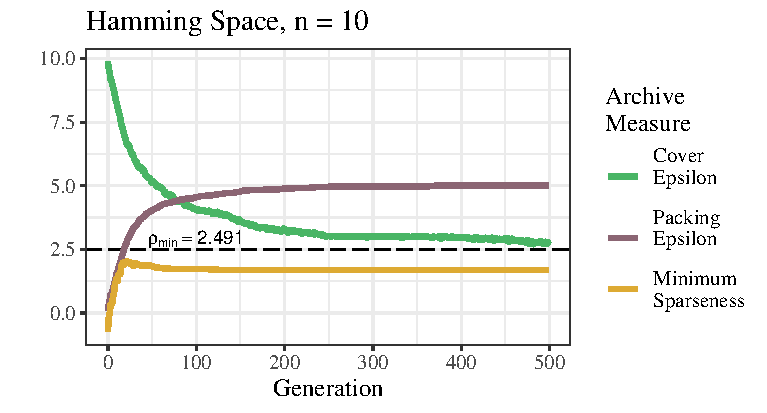
\includegraphics[width=0.75\textwidth]{Figures/hamming-500-n10-NOPOP.pdf}
  \caption{\label{fig:hamming:nopop:n10} SNSEA applied to a Hamming space with $n=10$ and $\rho_{min} = 2.491$ averaged over 50 independent trials.}
\end{figure}

We can see from Figure~\ref{fig:hamming:nopop:n10} that, indeed, the \chl{$\;\;\;\;$R1DC2}{}{coverage} of the Hamming space decreases steadily and the packing increases steadily.  This experiment clearly shows SNSEA converging to an $\epsilon$-net.  The internal sparseness measure also levels off with the other two curves.  These results are independent but consistent with \citep{Wiegand2020flairs}.  

Now let's see what \chl{$\;\;\;\;$R1DC2}{}{coverage} convergence looks like over different values of $n$ ($n\in\{6, 8, 10, 12, 14\}$).  Figure~\ref{fig:hamming:nopop:sm} below shows that in all cases, the algorithm appears to converge in terms of the \chl{$\;\;\;\;$R1DC2}{}{coverage} epsilon measure.
%
\begin{figure}[h]
  \center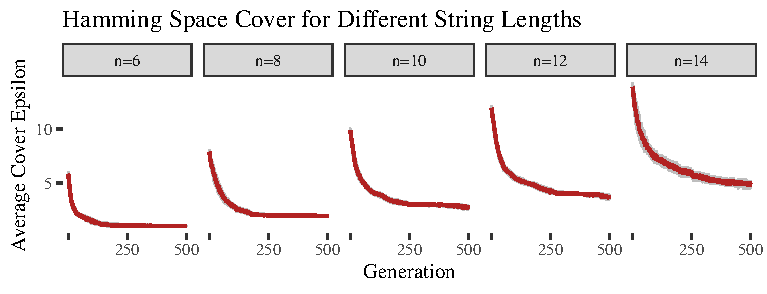
\includegraphics[width=0.9\textwidth]{Figures/hamming-500sm-NOPOP.pdf}
  \caption{\label{fig:hamming:nopop:sm} Coverage values for SNSEA applied to a Hamming space with $n$ ($n\in\{6, 8, 10, 12, 14\}$ averaged over 50 independent trials.}
\end{figure}

To determine whether these algorithms are indeed converging, we conducted the following experiment.  For each trial, we kept track of the lowest \chl{$\;\;\;\;$R1DC2}{}{coverage} value found and insisted that the algorithm must conduct at least 50 generations, and further that it must continue for at least as many generations as it took to first uncover that value without finding a lower value.  In other words, if it took 121 generations to find the lowest \chl{$\;\;\;\;$R1DC2}{}{coverage}, then we continued the algorithm until \emph{at least} generation 242 unless a new \chl{$\;\;\;\;$R1DC2}{}{coverage} value was found.  Moreover, we \emph{also} required that no additional points were added to the archive during the last half of the trial.

Our maximum number of generations was set to 5,000.  Anytime the \chl{$\;\;\;\;$R1DC2}{}{coverage} value found in a trial was discovered after to generation 2,500 \emph{or} any point was added to the archive after that point, we considered that trial to have \textsc{Not Converged}, otherwise the algorithm clearly \textsc{Converged} since \emph{doubling} the generation count to find a lower value did not help.  

In all trials of all values of $n$  for the Hamming space experiments, the SNSEA converged in the sense we just described.

While from the perspective of individual points in the space, one might be led to believe anecdotally that the process is divergent (the archive grows steadily until the space is filled), empirically we can see that the search is occurring at the level of the \emph{archive} space, not the individual point space.  In that sense, the process is clearly convergent\,---\,the SNSEA's archive converges in terms of \emph{\chl{$\;\;\;\;$R1DC2}{}{coverage}} in Hamming space.  Indeed, progress \emph{slows down} as saturation is approached.


%------------------------------------------------------------------------------------
\subsection{SNSEA Converges in Bounded Euclidean Space}
\label{subsec:bounded}
Again, it is easy to construct an example illustrating that bounded Euclidean spaces can converge.  We consider $d=5$, $\rho_{min} = 0.2$, $\sigma=0.1$, and a max generation of 500.  We ran 50 independent trials and again reported the mean values for our packing, \chl{$\;\;\;\;$R1DC2}{}{coverage}, and min sparseness approximations for each generation.  
 %
\begin{figure}[h]
  \center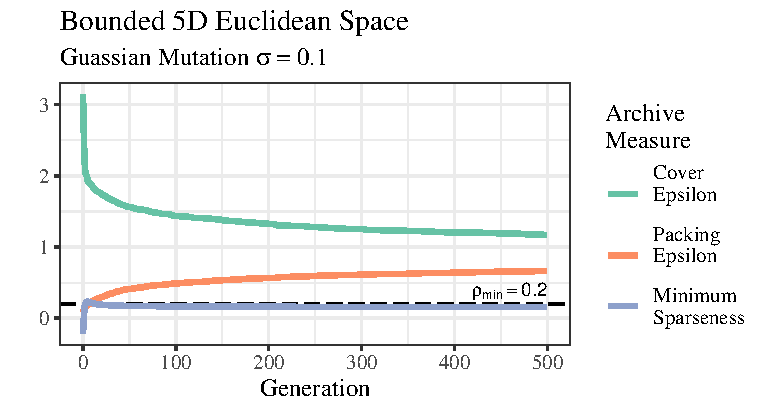
\includegraphics[width=0.75\textwidth]{Figures/bounded-s01-r02-NOPOP.pdf}
  \caption{\label{fig:bounded:nopop:0103} SNSEA applied to a bounded 5-dimensional Euclidean space averaged over 50 independent trials.}
\end{figure}

Figure~\ref{fig:bounded:nopop:0103} clearly shows an example in which the SNSEA on a bounded 5D Euclidean space converges \emph{both} in terms of \chl{$\;\;\;\;$R1DC2}{}{coverage} and packing.  Indeed, the algorithm appears to be converging toward an archive that approximates an $\epsilon$-net over the bounded space.  

Now let's see what \chl{$\;\;\;\;$R1DC2}{}{coverage} convergence looks like over different values of $\sigma$ and $\rho_{min}$.  Figure~\ref{fig:bounded:nopop:sm} below shows that in all but one case, the algorithm appears to converge in terms of the \chl{$\;\;\;\;$R1DC2}{}{coverage} epsilon measure.  When $\sigma=0.1$ and $\rho_{min} = 0.6$ the algorithm never improves at all.  This is because the radius of likely changes due to mutation is too small to generate sufficiently different individuals to meet the minimum sparseness conditions.  When the ratio between $\sigma$ and $\rho_{min}$ is around 1:3 or 1:4, the algorithm appears to perform the best in terms of making steady progress in \chl{$\;\;\;\;$R1DC2}{}{coverage}.  This again highlights the fact that there is an important balance to be reached between mutation and the sparseness criterion.
%
\begin{figure}[h]
  \center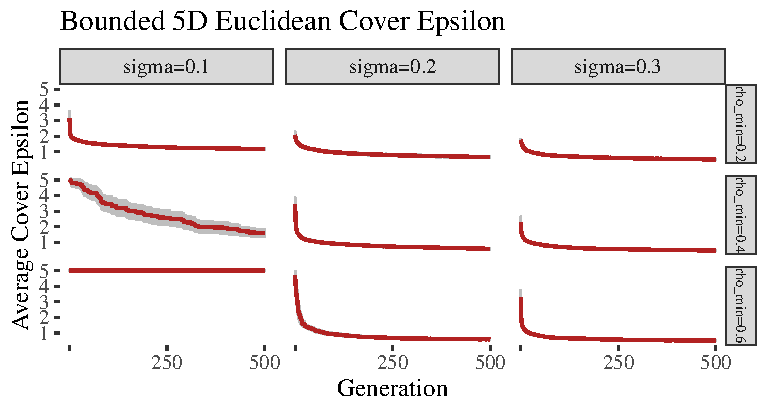
\includegraphics[width=0.75\textwidth]{Figures/bounded-500sm-NOPOP.pdf}
  \caption{\label{fig:bounded:nopop:sm} Coverage values for SNSEA applied to a bounded Euclidean space with $\sigma\in\{0.1,  0.2, 0.3\}$ and $\rho_{min} \in \{0.2, 0.4, 0.6\}$ averaged over 50 independent trials.}
\end{figure}

We considered a wide range of parameterizations of the algorithm, and in all cases the \chl{$\;\;\;\;$R1DC2}{}{coverage} can be observed to level off eventually (or fail to start).  To quantify this, we used the procedure described above:  each trial was allowed to continue until it took at least as long after finding the smallest \chl{$\;\;\;\;$R1DC2}{}{coverage} value or adding a new point to the archive.  If the algorithm accomplished these both before 2,500 generations, we considered it to have \textsc{Converged}.  Figure~\ref{fig:bounded:nopop:conv} below shows that in almost all cases, these conditions were met.  Even in the handful of cases where it did not meet, there were always more than 1,500 generations of stagnation before we gave up at generation 5,000.  
%
\begin{figure}[h]
  \center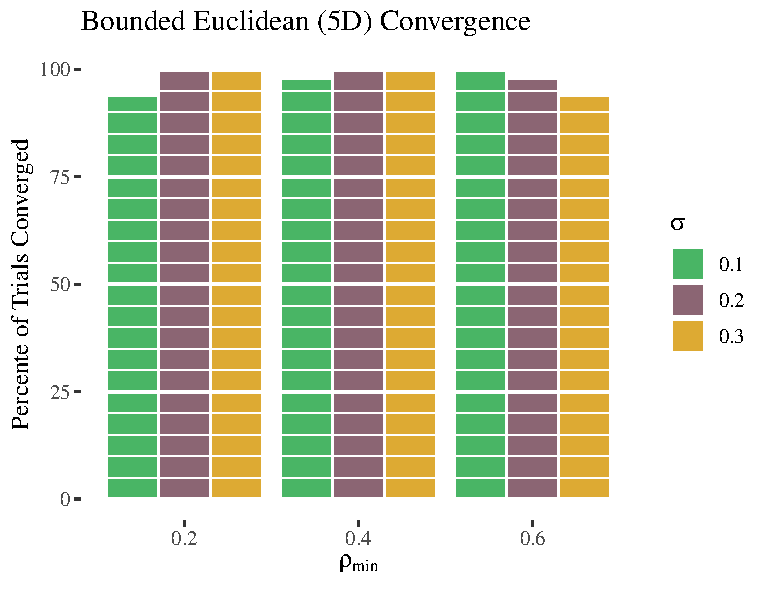
\includegraphics[width=0.6\textwidth]{Figures/bounded-conv-NOPOP.pdf}
  \caption{\label{fig:bounded:nopop:conv} Convergence percentages over 50 trials for the SNSEA operating over different $\sigma$ and $\rho_{min}$ values on a bounded Euclidean space.}
\end{figure}

Knowing that the SNSEA converges in bounded spaces is useful! We can implement approximations of \chl{$\;\;\;\;$R1DC2}{}{coverage} and packing in our algorithm, and when we see that an $\epsilon$-net is formed either stop the search or reset the archive to enable the search to explore new archive configurations.  


%------------------------------------------------------------------------------------
\subsection{SNSEA Can Converge in Unbounded Spaces}
\label{subsec:unbounded}

It should be noted that unbounded spaces present a particular challenge to novelty search algorithms \citep{LehmanStanley2008ssls,Doncieux2019gecco}.  Perhaps it is obvious that any bounded space will eventually be saturated by the archive?  What the above examples do, though, is illustrate that if your understanding is that novelty search is \emph{diverging until} it runs into the ``walls'' of the bounded space, then you may be looking at the process incorrectly:  The processes are \emph{converging} right from the beginning of the optimization, and the resulting archive is implicitly a local optimum (an $\epsilon$-net).

Still, it is constructive to look at unbounded spaces because we may be able to disentangle some misunderstandings.  For one, there appears to be the claim that because the space cannot be saturated, novelty search can have problems \citep{LehmanStanley2008ssls,Doncieux2019gecco}.  But saturation is not the issue.  Even in the unbounded case, there are parameterizations where the algorithm will converge in every sense of the word.  Figure~\ref{fig:unbounded:nopop:0102} illustrates such an example, where $\sigma=0.1$, $\rho_{min}= 0.2$, $d=5$, and the algorithm is run to 500 generations.  The space is completely unbounded.  While packing can still be estimated as it was above, \chl{$\;\;\;\;$R1DC2}{}{coverage} cannot be since the space is infinitely large.  To address this, we assume that the search will (with high probability) remain within the bound $\pm\sigma\cdot maxGen$ in all dimensions, and we estimate \chl{$\;\;\;\;$R1DC2}{}{coverage} as above but inside that region.  We also confirmed that though any 5D point was \emph{possible} in principle, in all runs none were generated outside that region.  Again, 50 independent trials were performed.
%
\begin{figure}[h]
  \center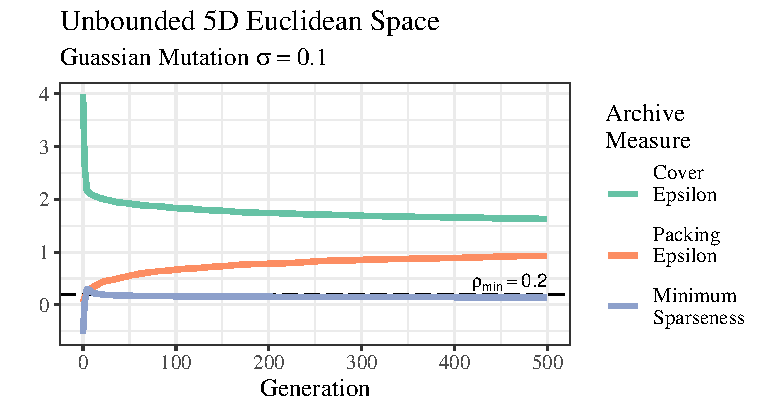
\includegraphics[width=0.75\textwidth]{Figures/unbounded-s01-r02-NOPOP.pdf}
  \caption{\label{fig:unbounded:nopop:0102} SNSEA applied to a bounded 5-dimensional unbounded Euclidean space averaged over 50 independent trials when $\sigma=0.1$ and $\rho_{min}=0.2$.}
\end{figure}

This process asymptotes toward an $\epsilon$-net just as in the bounded case.  Unbounded Euclidean spaces do offer an opportunity that bounded spaces do not:  The ability to keep adding new points on the \emph{outside} of the known, explored region.  Specifically, when the mutation $\sigma$ and $\rho_{min}$ are relatively far apart but $\rho_{min}$ is not so large that no progress can occur, then we can exacerbate the problem that occurs where large archive sizes make the algorithm increasingly unlikely to select points close enough to the surface of the archive that mutation has a reasonable probability to generate a point that will meet the sparseness criterion.  That is, we can create a scenario where new points on the edges of the known, explored space are very occasionally produced, and though they do not fundamentally change the ratio of the space that is \emph{covered} they do increase the largest pair-wise distance of points in the archive.
%
\begin{figure}[h]
  \center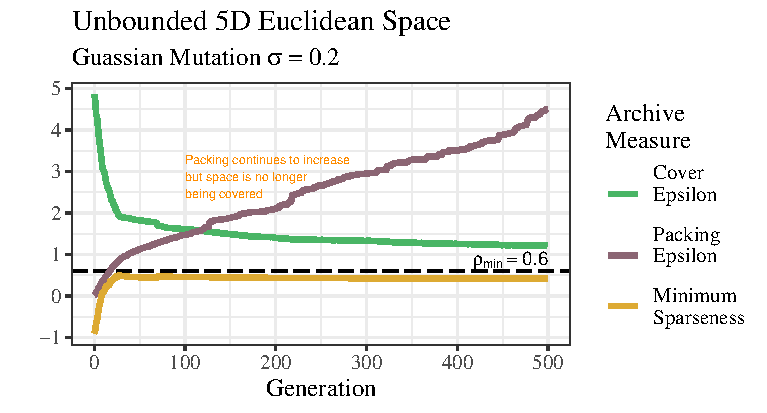
\includegraphics[width=0.6\textwidth]{Figures/unbounded-s02-r06-NOPOP.pdf}
  \caption{\label{fig:unbounded:nopop:0206} SNSEA applied to a bounded 5-dimensional unbounded Euclidean space averaged over 50 independent trials when $\sigma=0.2$ and $\rho_{min}=0.6$.}
\end{figure}

In Figure~\ref{fig:unbounded:nopop:0206} we see a situation in which \chl{$\;\;\;\;$R1DC2}{}{coverage} is converging but packing appears to be steadily increasing.  Indeed, though \chl{$\;\;\;\;$R1DC2}{}{coverage} appears to converge in most or all parameterizations, some parameterizations will lead to an apparent continual increase in the packing.  Though once the $\epsilon$-net is formed, the algorithm continues to occasionally add new points, these points are not substantively improving how the archive \emph{represents} the space\,---\,we're not really any closer to potential important points (e.g., a solution).  A local optimum has been identified by the algorithm, it has converged into that local optimum, and now it is making small fine-tuning changes to move closer to true locally optimal archive configuration strictly in terms of packing. This is analogous to a traditional real-valued EA maximizing a function like $f(x)=3x - 2$: once the top of the ridge is found, the EA will continue to produce new $x$ values that give larger $f(x)$.  Whether one calls this ``convergence'' or ``divergence'' depends on one's point of view; however, the SNSEA process \emph{is} optimizing against the packing/\chl{$\;\;\;\;$R1DC2}{}{coverage} objectives, regardless.

Again, we examine \chl{$\;\;\;\;$R1DC2}{}{coverage} convergence across different values of $\sigma$ and $\rho_{min}$.  Figure~\ref{fig:unbounded:nopop:sm} below shows that (again) in all but one case, the algorithm appears to converge in terms of the \chl{$\;\;\;\;$R1DC2}{}{coverage} epsilon measure.  As in the bounded case, when the ratio between $\sigma$ and $\rho_{min}$ is around 1:3 or 1:4, the algorithm appears to perform the best in terms of making steady progress in \chl{$\;\;\;\;$R1DC2}{}{coverage}.  
%
\begin{figure}[ht]
  \center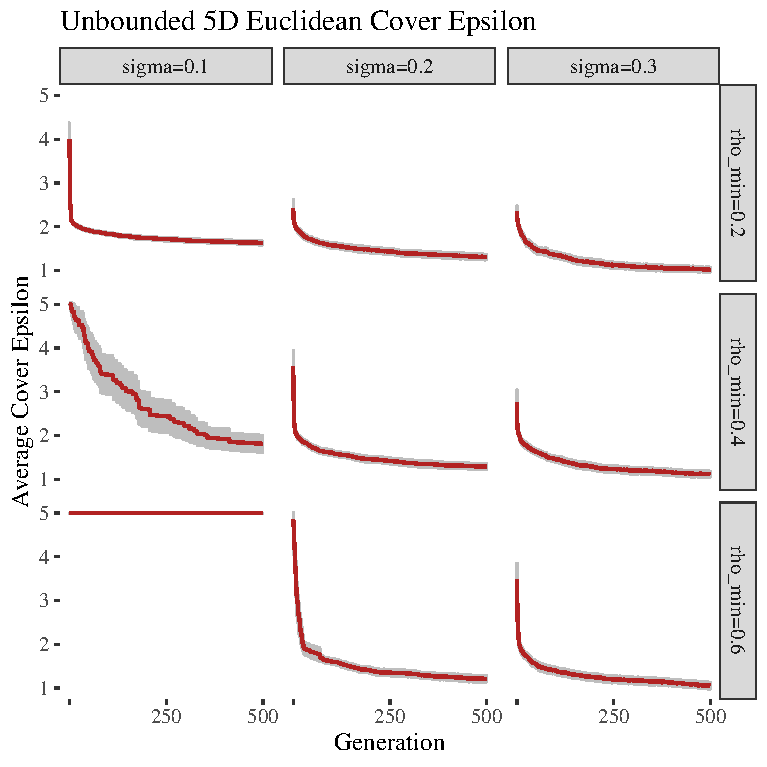
\includegraphics[width=0.75\textwidth]{Figures/unbounded-500sm-NOPOP.pdf}
  \caption{\label{fig:unbounded:nopop:sm} Coverage values for SNSEA applied to an unbounded Euclidean space with $\sigma\in\{0.1, 0.2, 0.3\}$ and $\rho_{min} \in \{0.2, 0.4, 0.6\}$ averaged over 50 independent trials.}
\end{figure}

Figure~\ref{fig:bounded:nopop:conv} below shows that in almost all cases, convergence conditions were met.  As before, even in the few of cases where it did not meet, there were always more than 1,500 generations of stagnation before we gave up at generation 5,000.  
%
\begin{figure}[ht]
  \center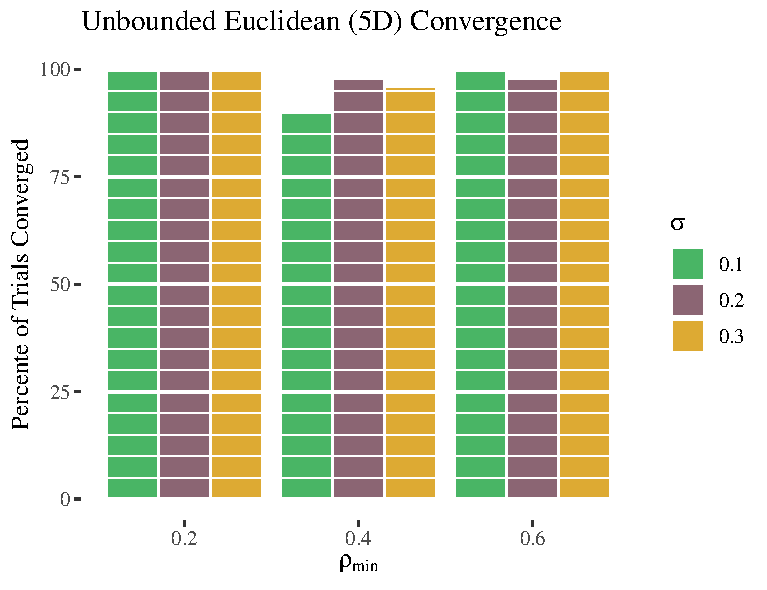
\includegraphics[width=0.75\textwidth]{Figures/unbounded-conv-NOPOP.pdf}
  \caption{\label{fig:bounded:nopop:conv} Convergence percentages over 50 trials for the SNSEA operating over different $\sigma$ and $\rho_{min}$ values on an unbounded Euclidean space.}
\end{figure}

To be clear:  We \emph{do not claim} that the SNSEA \emph{never} diverges, nor do we ascribe any quality (good or bad) to whether it \emph{should} converge or diverge.  We merely note that it \emph{does} converge in many cases.  More importantly, there are constructive things to learn about this observation.  For example, it's clear that balancing mutation and the sparseness criterion is very important.  %We will address this further in the discussion.


%====================================================================================
\section{The PSNSEA Optimization Process}
\label{sec:resultpsnesea}

Our population-based SNSEA is a lot more like a traditional novelty search algorithm:  Child individuals are selected from among the parent population individuals and the \emph{most novel} survive, while we also continue to update an ever-growing archive of individuals that meet our sparseness criterion.  In this section, we consider empirical results of such an algorithm.

\citet{Wiegand2021flairs} demonstrated that population-based SNSEAs can converge in the sense that we defined above; however, that work had a couple of limitations.  First, the paper considered unbounded spaces, spaces for which novelty search enthusiasts have already indicated may be less suitable for such methods \citep{LehmanStanley2008ssls}.  Second, the algorithm used $(\mu+\lambda)$ selection dynamics in order to drive home the point that convergence was at least \emph{possible}.  For the current paper, we consider bounded spaces and use less aggressive selection dynamics.


%------------------------------------------------------------------------------------
\subsection{PSNSEA Converges Quickly in Bounded Spaces}
\label{subsec:psnsea:bounded}

Figure~\ref{fig:bounded:mu2lam8:0102} illustrates such an example, where $\sigma=0.1$, $\rho_{min}= 0.2$, $d=5$, and the algorithm is run to 500 generations.  In this case, $\mu=2$ and $\lambda=8$.  Again, 50 independent trials were performed.  As with previous examples, the algorithm minimizes \chl{$\;\;\;\;$R1DC2}{}{coverage} and maximizes packing.  Indeed, this appears to happen much faster than for the SNSEA, which is consistent with the prior study.
%
\begin{figure}[h]
  \center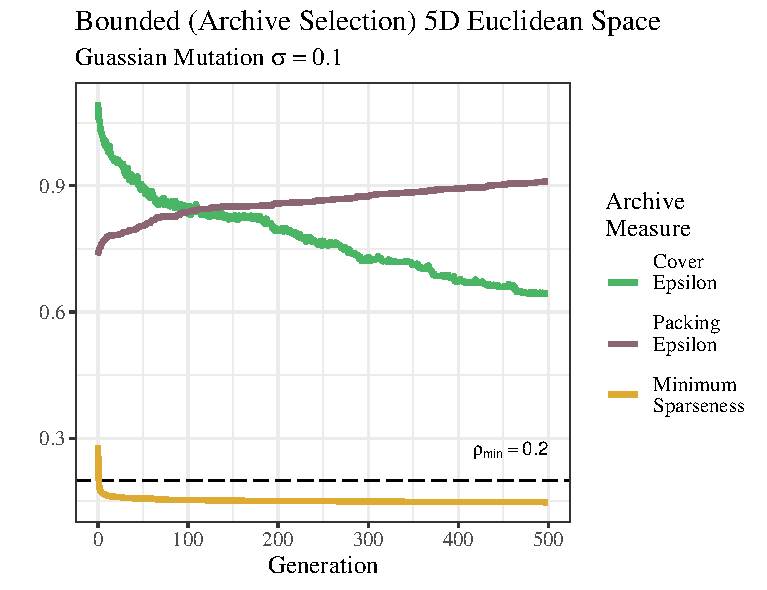
\includegraphics[width=0.75\textwidth]{Figures/bounded-500-s01r02-mu2lam8.pdf}
  \caption{\label{fig:bounded:mu2lam8:0102} PSNSEA applied to a bounded 5-dimensional unbounded Euclidean space averaged over 50 independent trials when $\sigma=0.1$, $\rho_{min}=0.2$, $\mu=2$, and $\lambda=8$.}
\end{figure}

For consistency, we examined the same parameter set of $\sigma$ and $\rho_{min}$ as in the previous section using $(2,8)$ selection dyanmics, Figure~\ref{fig:bounded:mu2lam8:sm}.  In all cases, \chl{$\;\;\;\;$R1DC2}{}{coverage} is minimized.  Convergence is slowest when $\sigma$ and $\rho$ are not to far apart.
%
\begin{figure}[t]
  \center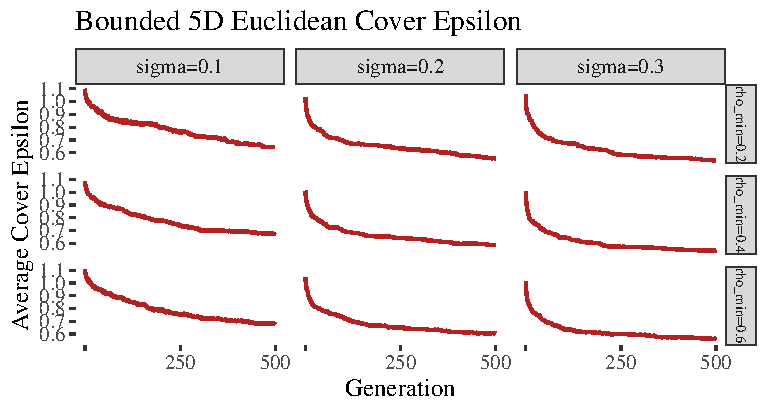
\includegraphics[width=0.75\textwidth]{Figures/bounded-500-sm-mu2lam8.pdf}
  \caption{\label{fig:bounded:mu2lam8:sm} Coverage values for PSNSEA applied to a bounded Euclidean space with $\sigma\in\{0.,  0.2, 0.3\}$ and $\rho_{min} \in \{0.2, 0.4, 0.6\}$ using $(2,8)$ selection dynamics averaged over 50 independent trials.}
\end{figure}


%------------------------------------------------------------------------------------
\subsection{PSNSEA Convergence for Different Population Sizes}
\label{subsec:psnsea:diffpop}

Of course, the population sizes will impact selection pressure and therefore convergence speed.  So we used the convergence test method described above to look at different values of $\mu$ and $\lambda$.  In all every trial of every parameterization the algorithm converged in the sense that the \chl{$\;\;\;\;$R1DC2}{}{coverage} estimate did not improve for at least double the number of generations it took to obtain that minimum.  Since it is not meaningful to plot the ratios of these, we instead plot the average generation at which this convergence was detected, shown in Figure~\ref{fig:bounded:pop:conv}.  
%
\begin{figure}[th]
  \center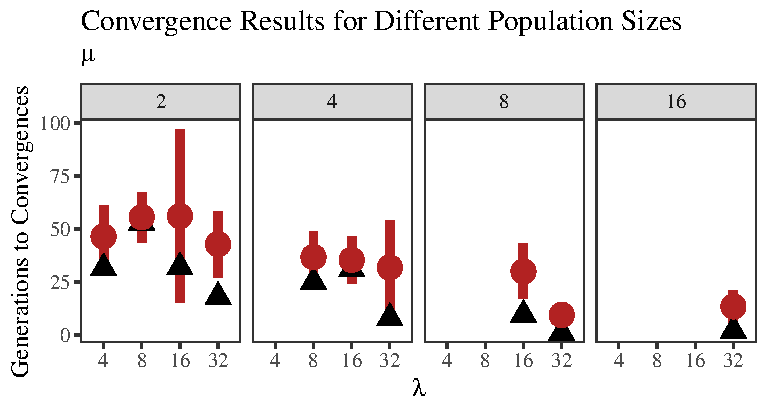
\includegraphics[width=0.75\textwidth]{Figures/bounded-conv-s02-r02.pdf}
  \caption{\label{fig:bounded:pop:conv} Convergence generation values for the PSNSEA applied to a bounded Euclidean space with $\sigma=0.2$, $\lambda=2$ for different population sizes.  The dots represent average ges over 50 independent trials, the triangle represents the median, and the lines are the 95\% confidence interval.}
\end{figure}

In general, the larger \emph{parent} the population, the faster the convergence.  This may seem obvious since it is qualitatively similar to what one expect from any EA for some problems, until one recalls the claims that novelty search diverges.  In fact, its dynamics in this respect do not appear to be that different from objective-based evolutionary strategies.  It's just in this case, the objective is to minimize \chl{$\;\;\;\;$R1DC2}{}{coverage}.


%------------------------------------------------------------------------------------
\subsection{Improving the PSNSEA}
\label{subsec:psnsea:improve}

One curious difference in terms of traditional dynamics is that the \emph{ratio} of child-to-parent population sizes doesn't seem to affect convergence speed.  There appears to be more going on than simple selection pressure.  In \citet{Wiegand2021flairs}, it was noted that the current populations in novelty search represent a current estimate for position in archive space, and it turns out that in some cases the PSNSEA populations do not represent the archive very well.  In that study, the severity of the $(\mu+\lambda)$ dynamics may have given a false sense of this property, so it's valuable to re-examine this under different conditions.

Recall the relationship between mutation and the sparseness metric discussed in Section~\ref{subsec:saturation}.  From that analysis, we know that we can greatly slow down the convergence of the archive to saturation by setting $\rho_{min}$ much lower than $\sigma$.  We will do this for our next experiment in order to better visualize the dynamics between the population and the archive in the PSNSEA.  Specifically, we use $\sigma=0.1$ and $\rho_{min}=0.001$) and apply $(2,8)$ selection dynamics.  Figure~\ref{fig:viz-archsell} illustrates a typical run over time.  We see that the child population (the points in red) are not particularly representative of the archive.  The point of novelty search is to spread out in the space, so this poor characterization of the archive slows down convergence.
%
\begin{figure}[h]
  \center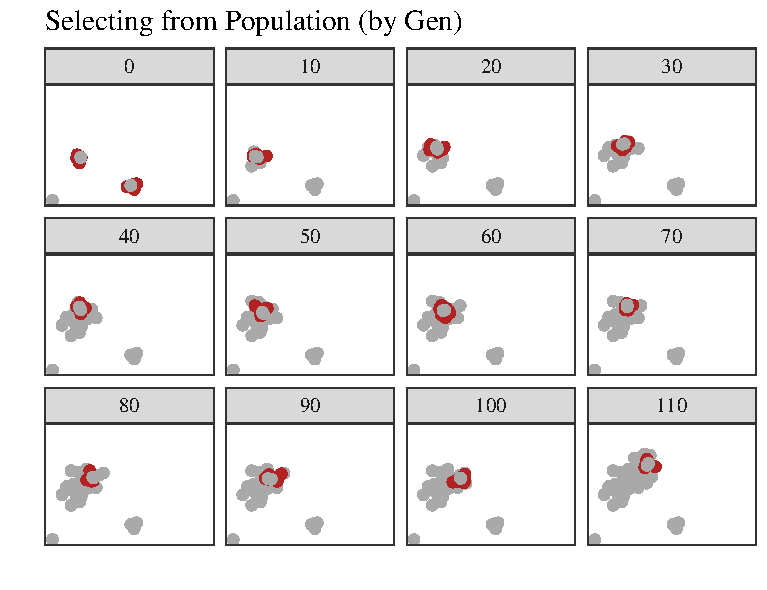
\includegraphics[width=0.6\textwidth]{Figures/viz-archive-and-pop-s01-r0001-mu16lam32-popsel.pdf}
  \caption{\label{fig:viz-popsel} Visualizing a $(2,8)$-PSNSEA applied to a bounded 2D Euclidean space with $\sigma=0.1$, $\rho_{min}=0.001$ over 110 generations.  The gray dots represent archive points, and the red dots represent the current children in that generation.}
\end{figure}

Understanding novelty search as a search through \emph{archive space} (rather than individual points) is key to addressing this issue.  The current population is a representation of archive space (as a whole), so it should be the case that improving this representation will speed up convergence\,---\,meaning the algorithm will cover the space faster.  If selecting points from the parent population leads to degenerate child population representations of the archive, then an easy way to improve that representation is to draw at least \emph{some} (say 75\% of) points directly from the archive itself, Figure~\ref{fig:viz-popsel}.   
%
\begin{figure}[h]
  \center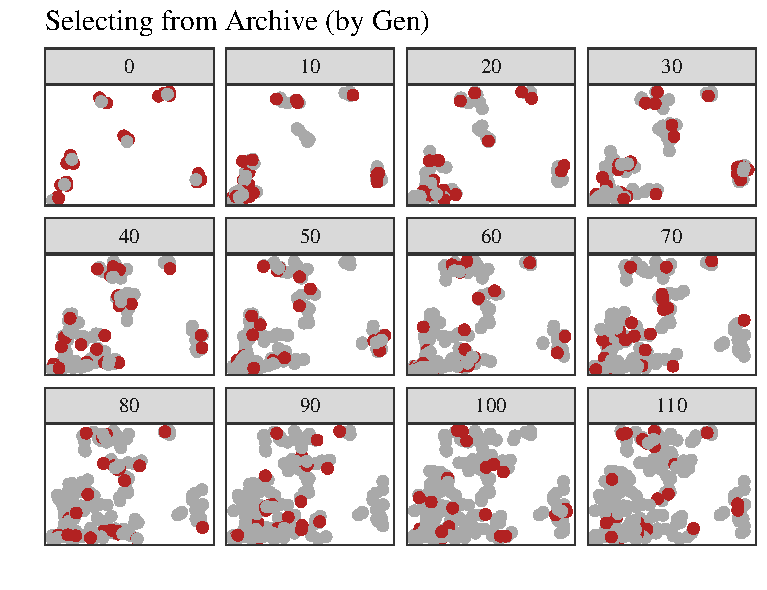
\includegraphics[width=0.6\textwidth]{Figures/viz-archive-and-pop-s01-r0001-mu16lam32-archsell.pdf}
  \caption{\label{fig:viz-archsell} Visualizing a $(2,8)$-PSNSEA applied to a bounded 2D Euclidean space with $\sigma=0.1$, $\rho_{min}=0.001$ over 110 generations.  The gray dots represent archive points, and the red dots represent the current children in that generation.  The algorithm is generating 75\% of children by drawing points from the archive.}
\end{figure}

This appears visually to be a big improvement.  But let's see how this affects one of our previous cases.  Figure~\ref{fig:bounded:viz:mu2lam8:0102} illustrates the identical case as the first one shown in this section:  a $(2,8)$-PSNSEA with $\sigma=0.1$ and $\rho_{min}=0.2$.  Except in this case, when selecting points to mutate to produce a child, we selected a point uniformly at random directly from the archive with 75\% probability.  If not drawn from the archive, the parent population was used as in all previous cases.
%
\begin{figure}[h]
  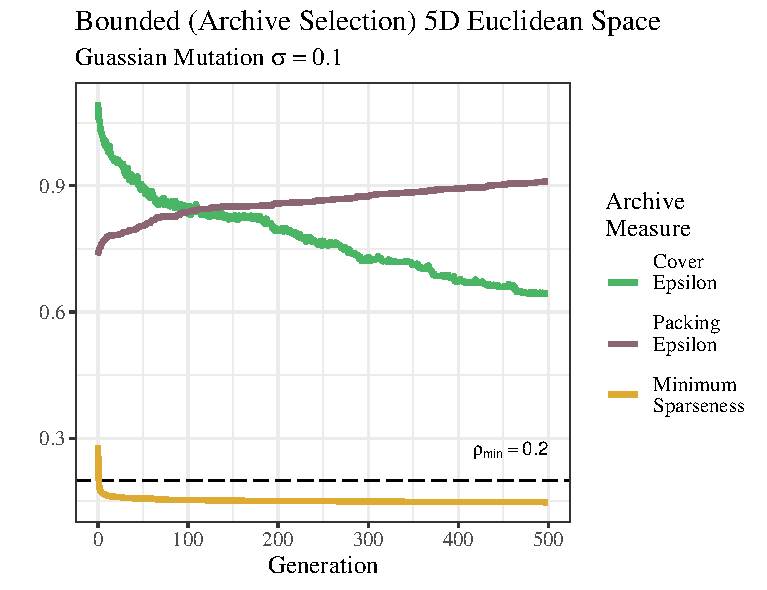
\includegraphics[width=0.48\textwidth]{Figures/bounded-500-s01r02-mu2lam8.pdf}
  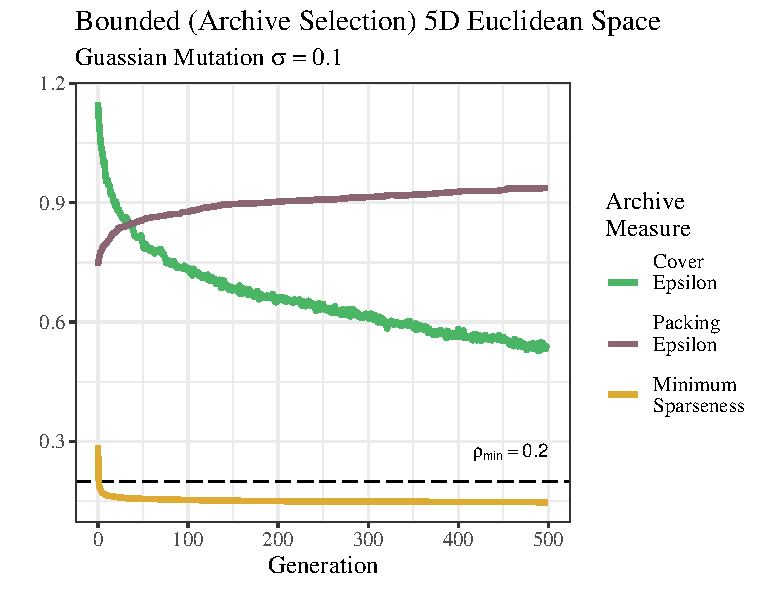
\includegraphics[width=0.48\textwidth]{Figures/boundedrv-500-vizexamp-mu2lam8-full.pdf}
  \caption{\label{fig:bounded:viz:mu2lam8:0102} PSNSEA applied to a bounded 5-dimensional unbounded Euclidean space averaged over 50 independent trials when $\sigma=0.1$, $\rho_{min}=0.2$, $\mu=2$, and $\lambda=8$.  On the left, all children come from parents drawn from the parent population.  On the right, there is 75\% chance each child comes from a parent drawn from the archive.}
\end{figure}

Archive selection drives the algorithm to a lower \chl{$\;\;\;\;$R1DC2}{}{coverage}, and it does so faster as well as more smoothly.  At least in this case, selecting individuals from the archive improves performance.  \chl{$\;\;\;\;$R2C6}{}{Indeed, treating the archive as the population itself is precisely the mechanism that the MAP-Elites method uses.  So our results represent an independent confirmation of this idea, as it applies to traditional novelty search.}

In general, we believe that finding ways for child samples to better represent the archive in terms of \emph{\chl{$\;\;\;\;$R1DC2}{}{coverage}} should improve novelty search performance.  Another example would be to maintain a subset of the archive that form a convex hull over the whole archive, and select points from that subset.  Monitoring \chl{$\;\;\;\;$R1DC2}{}{coverage} differences between the parent population and the archive may also provide triggers for when to make changes to selection methods.




%====================================================================================
\section{Discussion}
\label{sec:discussion}

%% RPW:  Add a discussion of reln b/w uncertainty min and novelty methods
%% RPW:  Also add discussion of why this isn't just an subjective view of dynamics & clarification of "divergence"

Novelty search can be a helpful algorithm for discovering complex objects.  Proponents espouse three critical components:  a sparseness metric and archive, generative representations, and distance measures in the actual solution space (e.g., behaviors) rather than genotype space.  The foundational work of understanding how novelty search works is only begun, though.  Since there are several claims about how novelty search explores spaces that exist in the literature, it is important to begin to address this.  The first idea to consider is the claim that novelty search is ``divergent'' and ``objectiveless''.  

In this paper, we consider only the first piece of the puzzle:  The sparseness metric and archive.  We use simplified variants of novelty search both with and without populations in order to concentrate on how the sparseness metric and the archive update criterion affect search dynamics.  We find that the most constructive view is that novelty search happens at the level of the \emph{archive space}, not the individual point space.  Looking at it this way is helpful because we can start to answer questions and make improvements to the algorithm and how we apply it.

First:  Is novelty search inherently ``objectiveless'', does it ``diverge''?  The answer to this question is very clearly, ``no.''   At least some novelty search methods are driven to spread out to \emph{\chl{$\;\;\;\;$R1DC2}{}{coverage}} the space, while trying to remain as efficiently \emph{packed} as possible.  Novelty search is driven to converge to an $\epsilon$-net in the sense defined by $k$-NN theory.  We do not claim that this is true of \emph{any} novelty search algorithm, just that the mere act of abandoning an external objective function in favor of a sparseness criteria does not make the search inherently divergent.  This is actually good news, since it means we can analyze the search process in similar ways as other optimization processes.  We simply have to change our perspective as to what is being searched (archive space) and what the objective is (\chl{$\;\;\;\;$R1DC2}{}{coverage}).

Second: Given it is optimizing, are there reasons to believe the algorithm will be particularly sensitive to certain parameter choices?  Indeed, there is an intrinsic relationship between mutation and the sparseness minimum.  For some problems, obtaining a good balance may be difficult.  Understanding the precise nature of this balance will be particularly difficult in true applications of novelty search since distance calculations will tend to be in \emph{behavior space}, not genome space.  This only exacerbates the problem that is inherent to the process.  Engineers that apply novelty search are warned that establishing a good balance between mutation and the sparseness minimum may well be challenging, and they should concentrate their attention on this during parameterization studies.

Third: If novelty search is optimizing for \chl{$\;\;\;\;$R1DC2}{}{coverage}, can we \emph{improve} that search?  We saw above, that at least in some cases it may be beneficial to draw points directly from the archive to improve population representation of the search space.  We speculate further that finding ways of making sure that the population remains near the \emph{boundaries} of the space will even further improve results by speeding up exploration of new portions of the space.

Finally, we might also ask:  Can novelty search get stuck in a local minima?  The answer is clearly that it can.  Consider a small, bounded space in which two archives exist that both saturate that space.  For simplicity of illustration, suppose $k=2$.  In such a case, no additional points may be added to either archive.  It's not hard to construct a pair of examples in which one of these archives is lower \chl{$\;\;\;\;$R1DC2}{}{coverage} than the other.  If so, then a search process that arrives at the larger \chl{$\;\;\;\;$R1DC2}{}{coverage} archive will be stuck and unable to improve.  

See Figure~\ref{fig:local:conv} for an illustration.  The space on the right will have lower \chl{$\;\;\;\;$R1DC2}{}{coverage} than the space on the left, but neither can admit more points.  This example is easy to generalize to larger $k$ and different packings of archives and $\rho_{min}$ values.  It can also be seen empirically with the fact that not every run of our experiments above converged to the same final \chl{$\;\;\;\;$R1DC2}{}{coverage} value.  
%
\begin{figure}[ht]
  \center\begin{tikzpicture}[scale=3]
    \pgfmathsetmacro{\r}{0.4}%
    \pgfmathsetmacro{\ll}{0.3}%
    \pgfmathsetmacro{\lu}{0.7}%
    \draw (0,0) -- (0,1) -- (1,1) -- (1,0) -- cycle;
    \draw[darkCB2, fill=darkCB2!50, opacity=0.3] (\ll, \ll) circle (\r);
    \draw[black, fill=black] (\ll, \ll) circle (0.02);
    \draw[darkCB2, fill=darkCB2!50, opacity=0.3] (\ll, \lu) circle (\r);
    \draw[black, fill=black] (\ll, \lu) circle (0.02);
    \draw[darkCB2, fill=darkCB2!50, opacity=0.3] (\lu, \ll) circle (\r);
    \draw[black, fill=black] (\lu, \ll) circle (0.02);
    \draw[darkCB2, fill=darkCB2!50, opacity=0.3] (\lu, \lu) circle (\r);
    \draw[black, fill=black] (\lu, \lu) circle (0.02);
    
    \draw[black, dashed] (\lu, \lu) -- (\lu, \lu+0.4);
    \node[anchor=west] at (\lu, 0.85) {\scriptsize $\rho_{min}$};
    
    \pgfmathsetmacro{\rl}{0.2}%
    \pgfmathsetmacro{\ru}{0.8}%
    \draw (2,0) -- (2,1) -- (3,1) -- (3,0) -- cycle;
    \draw[darkCB1, fill=darkCB1!50, opacity=0.3] (\rl+2, \rl) circle (\r);
    \draw[black, fill=black] (\rl+2, \rl) circle (0.02);
    \draw[darkCB1, fill=darkCB1!50, opacity=0.3] (\rl+2, \ru) circle (\r);
    \draw[black, fill=black] (\rl+2, \ru) circle (0.02);
    \draw[darkCB1, fill=darkCB1!50, opacity=0.3] (\ru+2, \rl) circle (\r);
    \draw[black, fill=black] (\ru+2, \rl) circle (0.02);
    \draw[darkCB1, fill=darkCB1!50, opacity=0.3] (\ru+2, \ru) circle (\r);
    \draw[black, fill=black] (\ru+2, \ru) circle (0.02);
    \draw[darkCB1, fill=darkCB1!50, opacity=0.3] (2.5, 0.5) circle (\r);
    \draw[black, fill=black] (2.5, 0.5) circle (0.02);
  \end{tikzpicture}
  
  \caption{\label{fig:local:conv} The figure on the left illustrates a bounded space saturated by a four point archive.  The figure on the right illustrates the same bounded space saturdated by a five point archive.  The figure on the right will have a lower coverage metric.}
\end{figure}

Our next step will be to examine how transformations of the genome space affect the efficiency with which novelty search can saturate bounded spaces.  In particular, most applications of novelty search involve measurements of behavior metrics that are of a much lower dimensionality than the genotypic space.  For example, the genes may encode the weights in a neural network while behavior may be measured as the end position of an agent in an environment.  This may have significant implications on the biases for how search progresses

\small

\bibliographystyle{apalike}
\bibliography{ref}


\end{document}
